\documentclass[class=article,crop=false]{standalone}
\usepackage[subpreambles=true]{standalone}
\usepackage{subcaption}
\begin{document}
\lecture
Here we will go into the early work that lead up to the development of \textbf{Quantum Mechanics} \\
Three concepts showed that eletromagnetic waves have particle-like properties:\\
\begin{enumerate}
	\item The photoelectric effect
	\item Thermal radiation (blackbody radiation)
	\item The Compton effect
\end{enumerate}

Energy is delivered not smoothly or continuously over a wave front, but rather in discrete bundles ("quanta") known as "photons".\\

\subsection{The Photoelectric Effect}
\subsubsection{Electromagnetic Waves}
EM Waves are predicted by Maxwell's equations, the electric and magnetic field each satisfy a wave equation. EM waves travel through vaccum with speed of light c:
$$ c = \frac{1}{\sqrt{mu_0 \epsilon_0}} $$
$\mu_0 = magnetic\ permeability,\ \epsilon_0 = electric\ permittivity$ \\
The electric and magnetic fields are perpendicular to each other, and perpendicular to the direction of the wave propagation. For a plane EM wave traveling in the position z direction: \\
$$ E = E_0 sin(kz - \omega t),\ B = B_0 sin(kz - \omega t) $$
$k = wave\ number, k = \frac{2 \pi}{\lambda}, \omega = angular\ frequency = 2\pi f $ \\
Magnitudes of an EM wave are related as $\frac{E_0}{B_0} = c$. EM waves carry energy, the energy flux is specified by the Poynting vector:
$$ S = 1/\mu_0 E \times B $$
For a plane wave:
$$ S = 1/\mu_0 \cdot E_0 \cdot B_0 \cdot sin^2 (kz - \omega t) \hat{k} $$
Where $\hat{k}$ is the unit vector in z-direction. \\

Note:\\
Power = energy per unit time\\
Energy flux = power per unit area\\
Intensity = average power per unit area (average energy per unit time and unit area)
\newpage
Assume we have a receiver to determine the EM power delivered by plane wave to recieved with sensitive area A: \\
$$ P = SA $$ If we can assume the reciever is perpendicular, we can ignore the vector component.
$$ P = 1/\mu_0 \cdot E_0 \cdot B_0 \cdot A \cdot sin^2(kz - \omega t) = \frac{1}{\mu_0 c} E_0^2 \cdot A \cdot sin^2(kz - \omega t) $$
Important takeaway is that intensity is proportional to the square of the amplitude and that something something time.\\

\subsubsection{Interference \& Diffraction}
Key property of waves is the principle of superposition.\\


\begin{figure}[h]
	\centering
	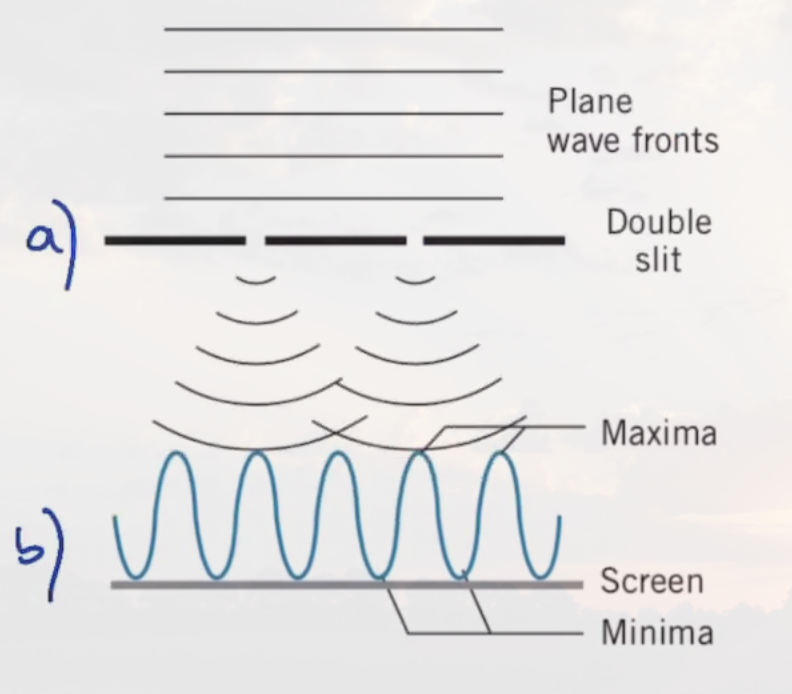
\includegraphics[width=.7\linewidth]{./Images/double_slit.png}
	\caption{Setup 1}
\end{figure}

Wave theory of light is insufficient though!

\subsubsection{Photoelectric Effect}
What is it? \\
Illuminate a metal surface with light - electrons can be emitted from the surface (1887). Work function: Minimum quantity of energy needed to remove an electron (material dependent). \\
When emmitted in this way, they're referred to as "photoelectrons".


\begin{figure}[h!]
	\centering
	\begin{subfigure}[b]{0.4\linewidth}
		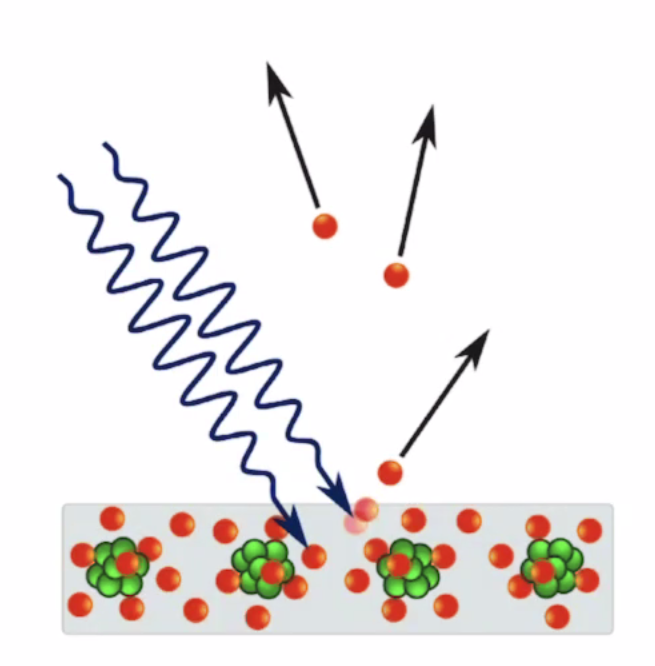
\includegraphics[width=.3\linewidth]{./Images/work_function.png}
		\caption{Setup 1}
	\end{subfigure}
	\begin{subfigure}[b]{0.4\linewidth}
		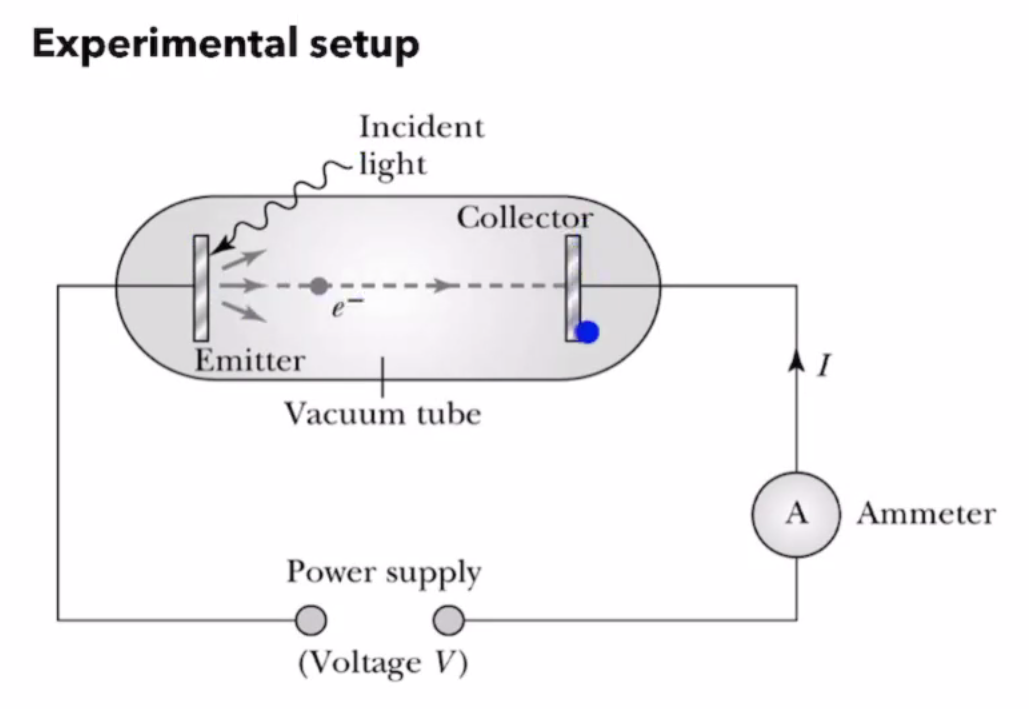
\includegraphics[width=.4\linewidth]{./Images/work_function_setup.png}
		\caption{Setup 1}
	\end{subfigure}
\end{figure}

Measure:\\
Rate of electron emission, measured as an electric current by an ammeter.\\
Maximum kinetic energy of the photoelectrons, measure by applying negative potential difference. \\
Electrons travelling from emitter to collector gain potential energy:\\
$$ \Delta U = q \Delta V = -e \Delta V (> 0,\ \Delta V\ is\ negative)$$
and lose the sam eamount of kinetic energy.\\

We can now determine the Maximum Kinetic Energy ($k_{max}$), by measuring the stopping potential ($V_s$).\\
$$ K_{max} = e V_s $$
Just large enough to stop the electrons from reaching the collector. \\

What are the expected results?
\begin{enumerate}
	\item For a given wavelength of light, as the intensity increases, the maximum kinetic energy of the photoelectrons should also increase.
	\item For a given wavelength of light, at low enough intensities there should be a time delay in electron emission.
	\item Electrons should be emitted for all wavelengths of light
\end{enumerate}

\begin{question}
None of these expectations were met by the experimental results.
\end{question}
Actual Experimental results:
\begin{enumerate}
	\item For a given wavelength of light, the amximum kinetic energy is independent of the intensity of the light source
	\item FIrst photoelectrons are emitted virtually instantaneously after the light source is turned on
	\item The photoelectric effect does not occur if the frequency of light is below a certain value
\end{enumerate}

\begin{question}
	This lead Einstien to formulate the quantum theory of the photoelectric effect
\end{question}

\begin{result}[Einstien's quantum theory of the photoelectric effect]
	Energy of an EM radiation is not countinously distributed across wave but concentrated in bundles: "quanta" (photons).\\
	Energy (E) of a photon associated with an EM wave: \\
	$$ E = hf $$
	$f$ = frequency of EM wave\\
	$h$ = Planck's constant = $6.626 \cdot 10^{-34} J \cdot s$ \\
	Because $f = c/\lambda \rightarrow E = \frac{hc}{\lambda}$
\end{result}
Because photons travel at the speed of light:
$$ E = pc $$
Where E is the energy and p is the momentum.
$$ p = \frac{E}{c} = \frac{\frac{hc}{\lambda}}{c} = \frac{h}{\lambda} $$

\subsubsection{Resulting interpretation of photoelectric effect}
One photoelectron released is due to encounter with a single photon. The entire energy of the photon is delivered instantaneously to the electron. If the photon energy is greater than the work function of a material, then a photoelectron is released. Otherwise, there is no photoelectric effect. \\

If a photon energy exceeds work function, excess energy is the kinetic energy of the electron: 
$$ K_{max} = E_{photon} - \phi = hf - \phi $$
Where $\phi$ = work function (depends on material).\\

This now explains why the maximum kinetic energy is independent of the intensity of the light source. I.e. Higher intensity means more photons striking surface, and more photoelectrons released, but all with the same maximum kinetic energy! There is no time delay, because the entire energy of the photon is delivered to the photoelectron. The photoelectric effect only occurs if the frequency of light is above a certain value, because the energy has to be greater than the work function, $E_{photon} > \phi,\ hf > \phi$. \\

Detailed tests of the photon theory were done by Millikan in 1915. He measured maximum kinetic energy (stopping potential) for different frequencies of light using sodium, and extracted Planck's constant (h).

\begin{figure}[h!]
	\centering
	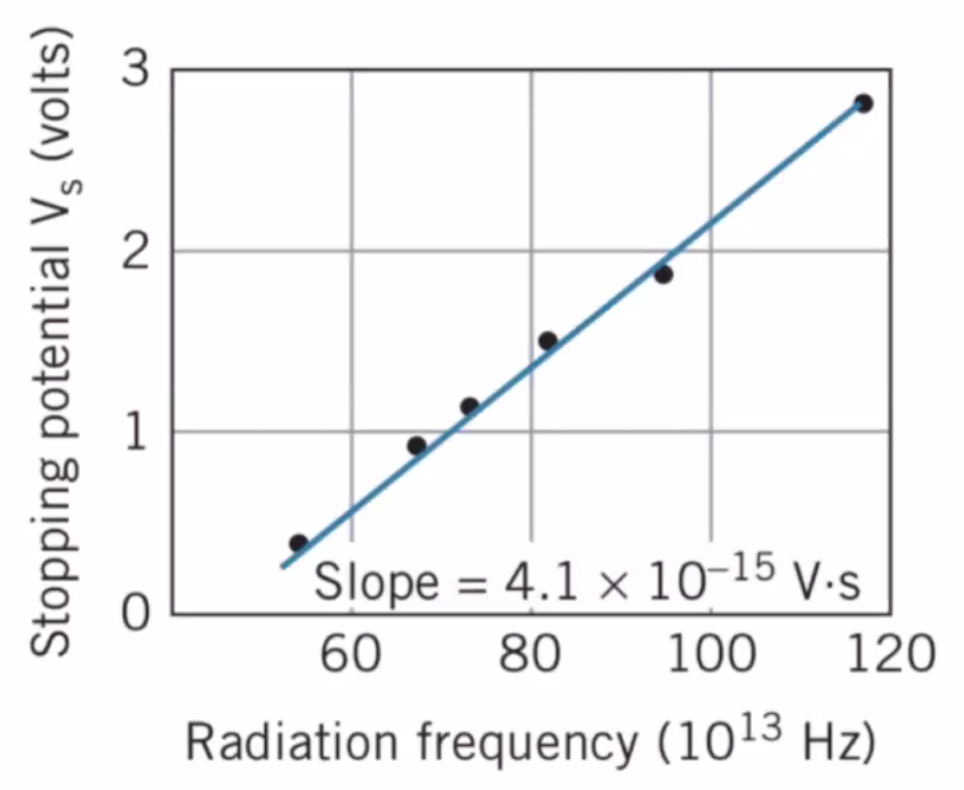
\includegraphics[width=.4\linewidth]{./Images/millikan.png}
	\caption{Millikan's results}
\end{figure}

\newpage
\begin{question}[Energy of a photon]
	What is energy and momentum of a photon of red light with wavelength 650 nm?
	\begin{answer}[Energy?]
		$$ E = hf = \frac{hc}{\lambda} $$
		Often convenient to use "eV".
		$$ hc = 1240 eV \cdot nm $$
		$$ E = \frac{1240}{650} \approx 1.9 eV $$
	\end{answer}
	\begin{answer}[Momentum?]
		$$ p = \frac{E}{c} = 1.9 eV/c $$
		Very convenient units!
	\end{answer}
\end{question}

\newpage
\begin{question}[Example]
	What happens if frequency is doubled while keeping photon emission rate unchanged?
	\begin{answer}[Frequency]
		Doubling the frequency will double the energy of the photons re. $e = hf$. Because $K_{max} = hf - \phi$ we will have a greater stopping potential, but current will be unchanged.
	\end{answer}
	What happens if the metal surface was replaced with one having a larger work function? 
	\begin{answer}[Work Function]
		If we have a greater work function this means that the maximum kinetic energy will be lower. If the work function exceeds the photon energy, then there will be no photoelectric effect.
	\end{answer}
\end{question}

\section{Thermal Radiation}

Thermal Radiation - Emission of electromagnetic waves by all objects with temperature greater than absolute zero.
Lightbulb, the sun, a human being, etc. However, a human body would emit light in the infrared range. \\
\subsubsection{Experimanetal results}
\begin{enumerate}
	\item Total intensity (I) radiated across all wavelengths is proportional to temperature (T) as:
		\begin{result}[Stefan's Law]
			$$ I = \sigma T^4 $$
			Where \[T\] = K, and the Stefan-Boltzmann constant $\sigma = 5.67 \cdot 10^{-8} \frac{W}{m^2K^u}$ and u refers to unit area.
		\end{result}
	\item Wavelength where the emitted intensity is maximal:
		$$ \lambda_{max} \propto 1/T $$
		\begin{result}[Wien's Displacement Law]
			$$ \lambda_{max} \cdot T = 2.8978 \cdot 10^{-3} m \cdot K $$
		\end{result}
\end{enumerate}

\subsubsection{Examples}
\newpage
\begin{question}[Example]
	At what wavelength does a human body emit maximum thermal radiation?
	\begin{answer}[Answer]
		$$ T \approx 310 K $$
		$$ \lambda_{max} = \frac{2.8978 \cdot 10^{-3} m \cdot K}{310 k} \approx 9.3 \mu m $$
		Indeed, the infrared range.
	\end{answer}
\end{question}

\begin{question}[Example]
	To what temperature must we heat an object to see its peak thermal radiation as visible light?
	\begin{answer}[Answer]
		if $\lambda_{max} = 700 nm:$\\
		$$ T = \frac{2.8978 \cdot 10^{-3} m \cdot K}{700 \cdot 10^{-9} m} $$
		$$\approx kfadslkjh $$
	\end{answer}
\end{question}

\subsection{Black-Body}
To simplify further analysis, we consider a "black-body":\\
\begin{result}[Black-body]
	Absorbs all radiation incident on it and reflects none of the incident radiation. \\
	(Note: A black-body can absorb energy which heats it up, and it will then emit its own radiation. But only its temperature determines the intensity and wavelength.)
\end{result}

We want to know how the intensity of the emitted radiation depends on wavelength.

\begin{result}[Classical Picture]
	Lord Rayleigh used classical theories of electromagnetism and thermodynamics to show that black-body intensity vs wavelength should be
	$$ I(\lambda) = \frac{2\pi c}{\lambda^4} kT $$
	This "Rayleigh-Jeans" formula is not accurate.
\end{result}
One major problem is that it fails badly to match eperimental data for low wavelengths.

\subsection{Quantum Theory of thermal radiation}

Planck assumed that the radiation in the blackbody was emitted by some sort of "oscillators", and used statistical methods recently developed by Boltzmann.

Planck's modification:\\
The cavity radiation originates from oscillations inside the cavidy walls. These oscillations can only have discrete values of energy:
$$ E_n = n \cdot \epsilon,\ n = 1,2,3,4...$$
These oscillators can absorb or emit energy only in discrete bundles ("quanta") of the fundamental quantum energy given by:\\
$$ \sigma = hf $$
$ h = Planck's constant = 6.63 \cdot 10^{-34} J\cdot s $
\begin{figure}[h!]
	\centering
	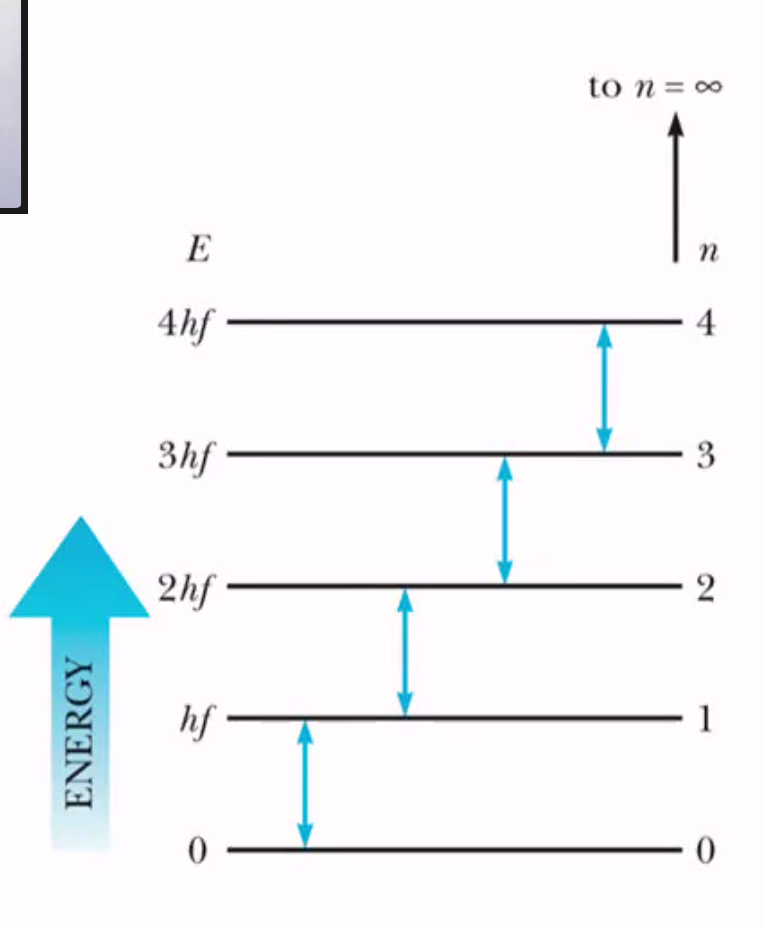
\includegraphics[width=.7\linewidth]{./Images/oscillators.png}
	\caption{Setup 3}
\end{figure}

\newpage
\begin{result}[Intensity as a Function of Wavelength]
	$$ I(\lambda) = \frac{2\pi hc^2}{\lambda^5} \cdot \frac{1}{e^{hc/\lambda KT} - 1} $$
	I: Intensity of radiation \\
	h: Planck's constant\\
	$\lambda$: Wavelength\\
	k: Boltzmann's constant\\
	T: Temperature
\end{result}

Stefan's law from Planck's law gives a relationship between Stefan-Boltzmann's constant ($\sigma$) and Planck's constant (h): \\
$$ \sigma = \frac{2\pi^5k^4}{15c^2h^3} $$
Found by integrating across all wavelengths. \\\\

Millikan obtained the value of Planck's constant using the photoelectric effect, measuring the maximum kinetic energy as a function of frequency( absorption of EM radiation). Planck determined the value of h using blackbody intensity data (emission of EM radiation).\\
\emph{These agreeing implies it is not an accident but a property of the EM field.} \\

\subsubsection{Cosmic Microwave Background (CMB)}
CMB is very close to a perfect black-body. 

\begin{figure}[h!]
	\centering
	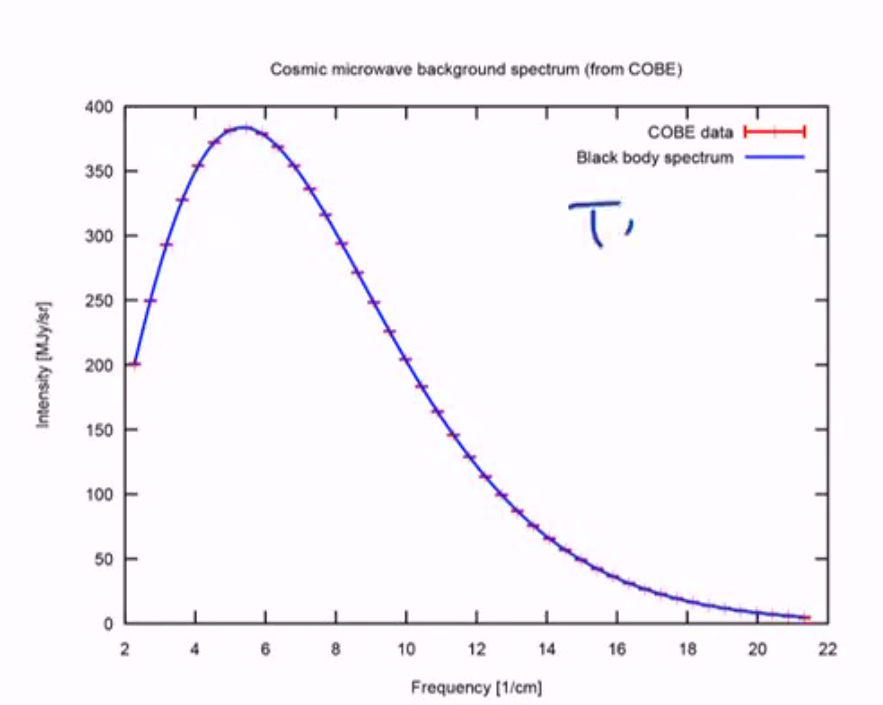
\includegraphics[width=.7\linewidth]{./Images/cmb.png}
	\caption{Setup 3}
\end{figure}
\newpage
Origin: 
\begin{itemize}
	\item In very early times, the Universe was filled with hot plasma of particles. These photons were constantly interacting with free electrons, "stopping" them.
	\item After some 380,000 years, Universe had expended and cooled to ~3000K, where electrons and protons could form hydrogen atoms
	\item Photons now free to roam!
	\item These photons fill the Universe today and are detected as the CMB!
	\item Blackbody spectra observed is that of T $\approx$ 2.7K because photon frequency we detect is greatly Doppler shifted (wavelength is "redshifted").
\end{itemize}

\begin{question}[Example: The sun as a blackbody]
	Treating the Sun as a blackbody (good approximation), and using that its radius is $7 \cdot 10^8 m$ (R), the average Earth-Sun distance is 1.5 $\cdot 10^{11} m\ (R_s)$, and the power per unit area from the Sun as measured on Earth is $W/m^2$. Estimate the surface temperature of the Sun.
	\begin{answer}[Answer]
		Need: connect $I(R_s) to I(R)$\\
		Conservation of energy:
		$$ I(R_s) \cdot 4 \pi R_s^2 = I(R) 4\pi R^2 $$
		$$ I(R_s) = I(R) \cdot \frac{R^2}{R_s^2} $$
		Can deduce that the surface temp T = $ I = \sigma T^4$
		$$ \sigma T^4 = I(R) \cdot \frac{R^2}{R_s^2} $$
		$$ T = (\frac{I(R)}{\sigma} \cdot \frac{R^2}{R_s^2} = \frac{1400 W/m^2}{5.67 \cdot 10^{-8}} \cdot \frac{1.5 \cdot 10^{11}}{7.0 \cdot 10^8} $$
		$ T \approx 5800 K $
	\end{answer}
\end{question}

\newpage
\section{The Compton Effect}

Finally shifted public support for Einstien's explanation of black-body radiation.\\

Scattering of radiation from lossely bound, nearly free electrons.\\

The classical wave picture would predict that scattered radiation is less energetic than incident radiation, and would have the same wavelength. \emph{the latter point failed in experiments}\\

Consider this process instead as the scattering of a photon - \\
An interaction between two particles, incident photon and electron off which it scatters. In the classical sense an interaction is a collision. \\

\begin{figure}[h!]
	\centering
	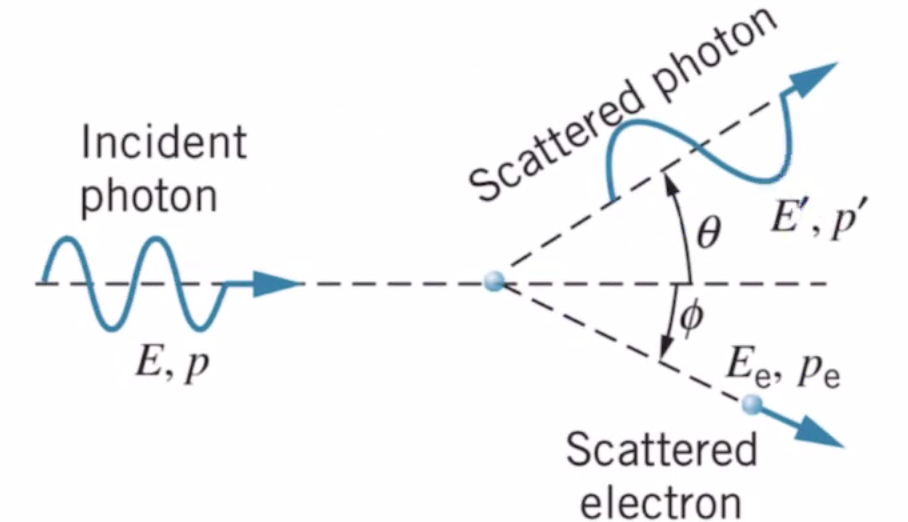
\includegraphics[width=.7\linewidth]{./Images/compton effect.png}
	\caption{Compton Effect}
\end{figure}

\begin{question}[Conservation laws for relativistic momentum and total energy]
	Energy: $ E + m_ec^2 = E' + E_e $ \\
	Momentum: \\
	Horizontal : $ p = p' cos(\theta) + p_e cos(\phi) $ \\
	Vertical : $ 0 = p' sin(\theta) - p_e sin(\phi) $ \\
	\begin{answer}[Eliminate $\phi$]
		$$ p_e cos\phi = p - p'cos\theta $$	
		$$ p_e sin\phi = p'sin\theta $$	
		$$ p_e^2(cos^2\phi+sin^2\theta) = p^2 + p'^2cos^2\theta - 2pp'cos\theta _ p'^2 $$
		$$ p_e^2 = p^2 + p'^2 - 2pp'cos\theta $$
	\end{answer}

	\begin{answer}[Eliminate $E_e$]
		$$ E_e = E - E' + mc^2 $$
		Note: $ E^2 = (mc^2)^2 + (pc)^2 $ \\
		$$ E_e^2 = (E-E')^2 + (m_ec^2)^2 + 2(E-E')m_ec^2 $$
		$$ (m_ec^2)^2 + (p_ec)^2 = (E-E')^2 + (m_ec^2)^2 + 2(E - E')m_ec^2 $$
		$$ (p_ec)^2 = (E-E')^2 + 2(E - E')m_ec^2 $$
		Plug part a into the expression.
		$$ p^2c^2 + p'^2c^2-2pp'c^2cos\theta = E^2+e'^2-2EE'+2(E-E')m_ec^2 $$
		Note: E = pc for a photon. $p^2c^2 = E^2, p'^2c^2 = E'^2$.
		$$ -2EE' cos\theta = -2EE' + 2(E-E')m_ec^2 $$
		\begin{result}[Compton Scattering]
			$$ 1/E' - 1/E = \frac{1}{m_ec^2}(1-cos\theta) $$
		\end{result}
		\begin{result}[Wavelength]
			$E = \frac{hc}{\lambda}$
			$$ \lambda' - \lambda = \frac{h}{m_ec}(1-cos\theta) $$
			$\lambda '$ : wavelength of scattered photon\\
			$\lambda $ : wavelength of incident photon\\
			The difference betweeen those two values depends on the angle. If the angle is 0. 
		\end{result}
	\end{answer}
\end{question}

Compton found that light scattered from a particle at rest is shifted in wavelength! This was viewwed as a direct and incontrovertible experimental evidence that light behaves as a particle (on a subatomic scale!) This particle is the photon (symbol $\gamma$).

\begin{answer}[Kinetic energy gained by the electron?]
	$$ E + m_ec^2 = E' + m_ec^2 + Ke \rightarrow E' + E $$
\end{answer}

\newpage
\begin{question}[Examples (Groups)]
	Why are x-ray photons used in the Compton experiment, rather than visible light photons? \\
	\begin{answer}[Three cases]
		\begin{enumerate}
			\item High energy rays from cobalt, $\lambda$ = 0.00106 nm.\\
				$$ \lambda' - \lambda = \frac{h}{m_ec}(1-cos\theta) $$
				$$ \lambda' - \lambda = \frac{6.63 \cdot 10^{-34}Js}{9.10938356 × 10{-31} kg}(1) = 7.274 \cdot 10^{-4} = 2.4277 nm $$

				The shift is substantially larger than the incident wavelength. \\
			\item Shift = 2.4277 nm (same regardless of incident wavelength), 0.0712 nm is the incident.\\
				This one is just right.

			\item Shift = 2.4277 nm (same regardless of incident wavelength), 546 nm nm is the incident.\\
				The shift in wavelength is very small compared to the incident wavelength.
		\end{enumerate}
	\end{answer}
	\begin{answer}[Binding energy]
		The binding energy will be very small compared to the energy of the x-ray.
		$$ hc/\lambda = a\ lot $$
	\end{answer}
\end{question}
\begin{question}[Photoelectric effect in Zinc]
	Photoelectrons released from zinc by ultraviolet light were stopped by a voltage of 4.3 V.
What is the maximum kinetic energy and speed of the photoelectrons?
\end{question}

\subsection{What is a photon?}
\begin{itemize}
	\item Just like an EM wave, photons move at the speed of light
	\item Photons have zero mass and zero rest energy
	\item Photons carry energy and momentum, related to the frequency/wavelength of EM waves
		$$ E = hf = \frac{hc}{\lambda} = pc \rightarrow p = \frac{h}{\lambda} $$
	\item Photons can be created or destroyed when radiation is emitted or absorbed
	\item They can collide with other particles, like electrons
\end{itemize}

\textbf{\emph{Wave-particle duality, light is neither a particle nor a wave, it is both.}}
Our failure to classify light as one or the other is more a failure of our vocabulary, as light is a "quantum particle".

\subsubsection{Connection between wave behavior and particle behavior of light}
Probability to observe photons is proportional to the electric field amplitude squared\\

\section{Atoms}
Around year 1900, evidence indicating that the atom was not a fundamental unit, but instead composed of smaller particles... \\
\subsection{Knowledge of atoms at the time}
\begin{itemize}
	\item Atoms are very small
	\item Atoms are stable (usually)
	\item Atoms are electrically neutral, but since they contain  electrons, there must be a corresponding net positive charge
		\begin{itemize}
			\item The electron was discovered, protons were not, but it was understood that some positive charge had to be present
		\end{itemize}
	\item Atoms can emit and absorb electromagnetic radiation
\end{itemize}

\subsubsection{Atomic Model 1904}
An early model of the atom was proposed by J.J. Thomson. It was known as the Thomson model (alternatively plum-pudding model), where protons and electrons were all mixed up together. Thomson thought an electron could vibrate about its equilibrium position when the atom was heated and produce electromagnetic radiation. \\
This would predict that light would scatter in a way inconsistent with observations.

\begin{figure}[h!]
	\centering
	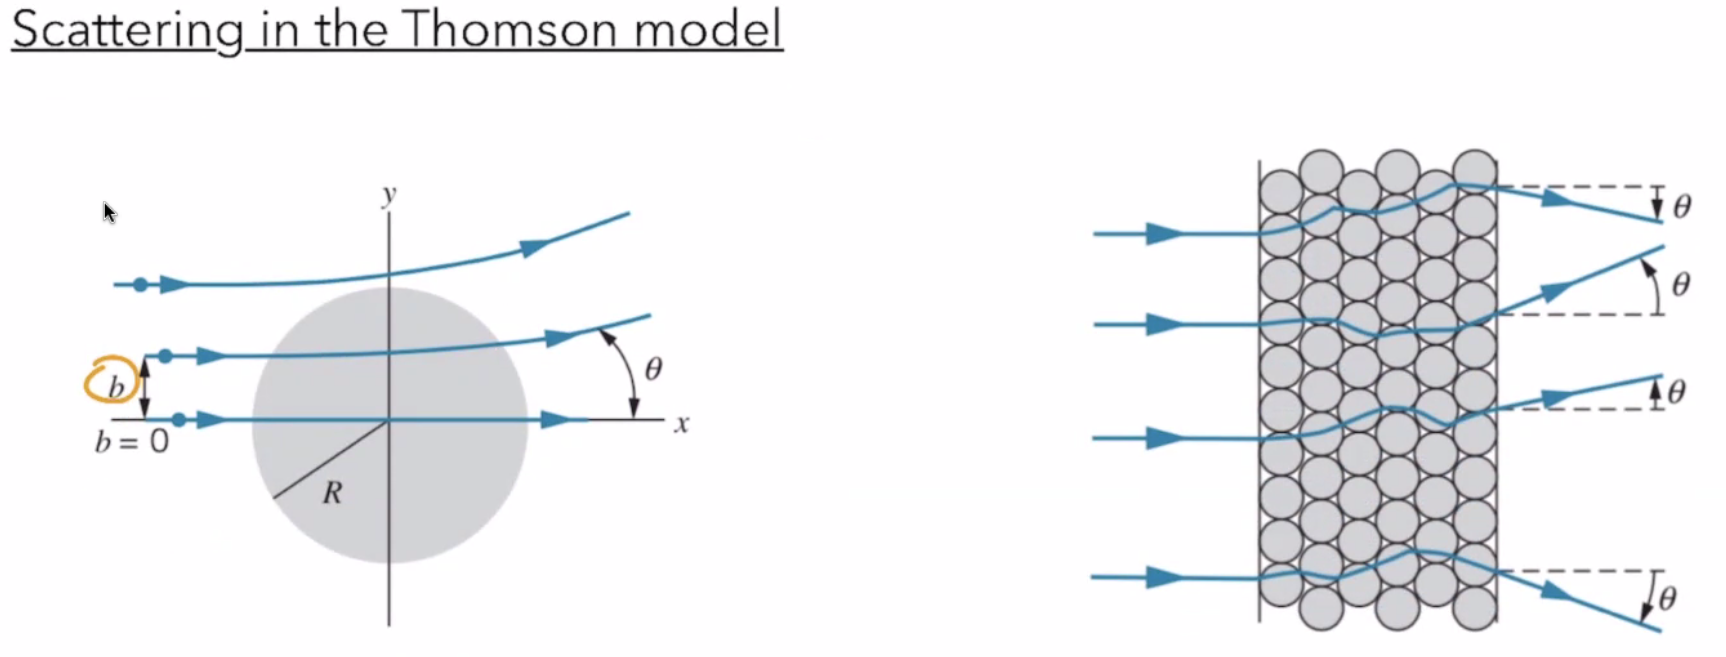
\includegraphics[width=1\linewidth]{./Images/thomson.png}
	\caption{Thomson}
\end{figure}

Tested with micrometer thick foil (n ~ $10^4$). Expected scattering angle would be about a degree, no scattering at large angles. 

\subsection{Rutherford Scattering}
1910 performed important scattering experiment in the laboratory of E. Rutherford, in order to stody the structure of matter. Alpha particles (He nucleus (+2e)) scattering by a thin gold foil. Observed a non-negligable scattering at very large angles.

\begin{figure}[h!]
	\centering
	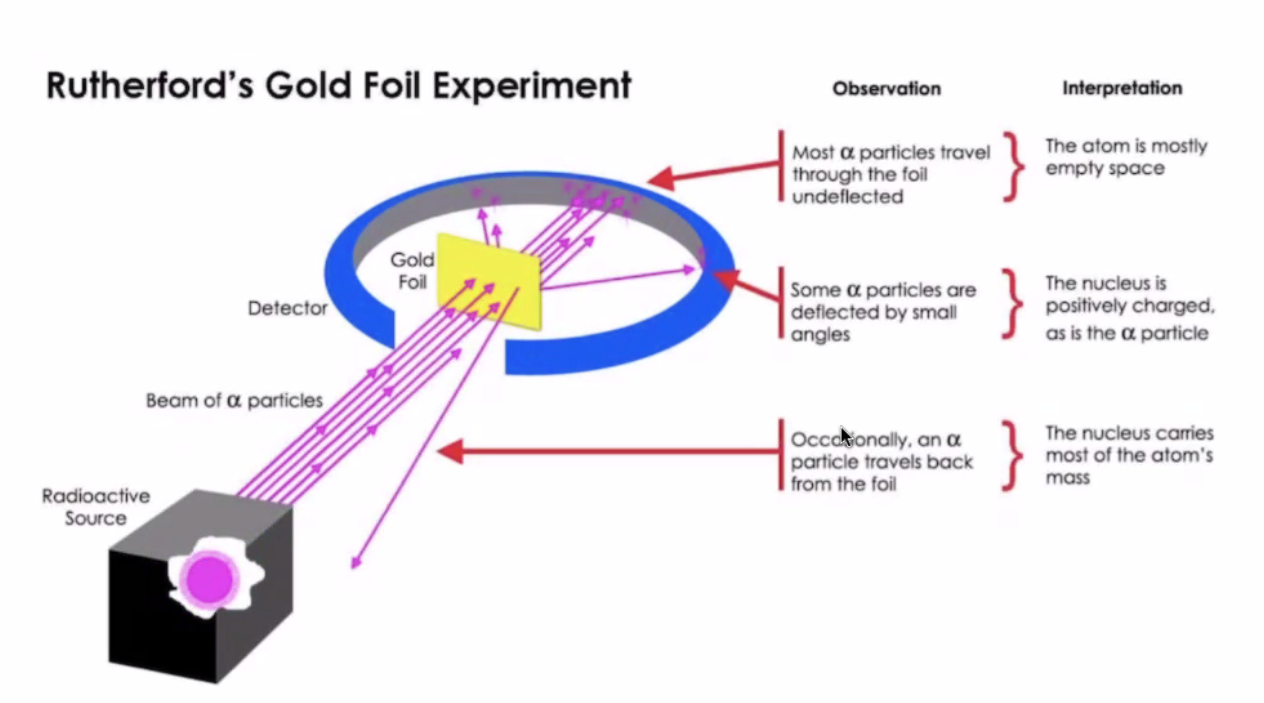
\includegraphics[width=1\linewidth]{./Images/rutherford.png}
	\caption{Rutherford}
\end{figure}

Lead to the realization that atoms were mostly empty space, with positive charge and mass concentrated in a very small region. This is known as the nucleus.

\subsubsection{Analysis}
Repulsive force experienced by projectile: 

\begin{figure}[h!]
	\centering
	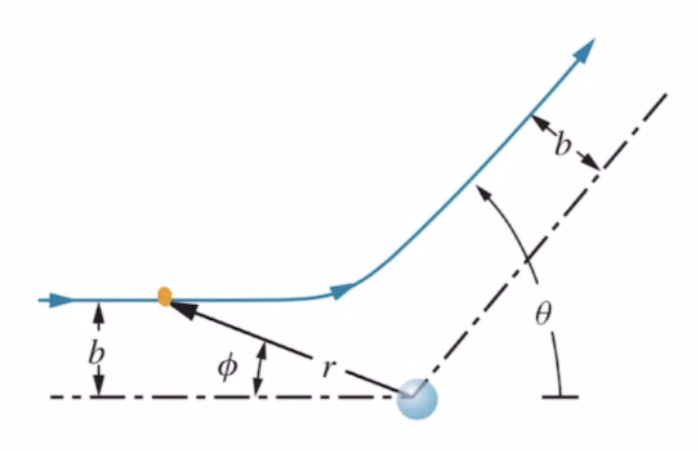
\includegraphics[width=.5\linewidth]{./Images/rscatter.png}
	\caption{Rutherford}
\end{figure}

$$ F = \frac{1}{4\pi \epsilon_0} \frac{|q_1||q_2|}{r^2} = \frac{(ze)(Ze)}{4\pi \epsilon_0r^2} $$

Assumptions:
\begin{enumerate}
	\item Electrons in the atom do not have any sizeable contribution to the scattering due to their small mass.
	\item Nucleus much more massive than the projectile such that it doesn't noticeably move during scattering process
\end{enumerate}

It can be shown that projectile follows a hyperbolic path:

$$ 1/r = 1/b\ sin \phi + \frac{zZe^2}{8\pi\epsilon_0b^2k}(cos\phi-1) $$
z, Z: electric charge of particle, nucleus \\
K: kinetic energy of particle

We can relate the impact parameter (b) to the scattering angle ($\theta$):
$$ b = \frac{zZ}{2k} \frac{e^2}{4\pi\epsilon_0} cot(\frac{\theata}{2}) $$
Where 
$$ \frac{e^2}{4\pi\epsilon_0} = 1.44 eV*nm $$

What fraction of projectiles are scattered at angles greater than some particular value?
Some impact parameter $b_0$ corresponds to a given angle $\theta_0$. A projectile scattered at $\theta > \theta_0$ means it must have $b<b_0$. \\
What fraction has that? \\
\begin{enumerate}
	\item Single layer of atoms:\\
		$$  f = \frac{\pi b_0^2}{\pi R^2} $$
	\item Multiple layers of atoms: (Due to technological constraints)\\
		Volume of the target :\\
		$$ V = At $$
		\# Atoms in this volume:\\
		$ \rho = density $
		$ N = n_{moles} \cdot N_A = \frac{m}{M} \cdot N_A $ \\
		$\ \ = \frac{\rho V}{M} \cdot N_A = \frac{\rho At}{M} \cdot N_A$
		\# atoms per unit volume: \\
		$n = \frac{N}{V} = \frac{\rho N_A}{M}$\\
		Incident projectile sees: n*t nuclei/unit area \\
		Effective area that each nuclei contributes will be $\frac{1}{n\cdot t}$\\
		Fractions of projectiles that fall within $\pi b_0^2$:
		$$ f = \frac{\pi b_0^2}{1/(ut)} = nt\pi b_0^2 $$
		Fraction of projectiles that scatter with angle $> \theta_0$:
		$$ f(\theta > \theta_0) = f(b < b_0) = nt\pi b_0^2 $$
\end{enumerate}


\begin{question}[Example]
	We have a thin gold foil (2.0$\cdot 10^{-4}$) off which alpha particles with kinetic energy of 8 MeV are scattered. \\
	What fraction are scattered at angles larger than 90 $\degrees$
	\begin{answer}[Scattering at 90$\degrees$]
		$$ b = \frac{zZ}{2K} \frac{e^2}{4\pi\epsilon_0} cot(\theta/2) $$
		z: 2\\
		Z: 79\\
		K = 8 MeV\\
		$\theta$ = 90$\degrees$\\
		$$ b \approx 14 fm $$
	\end{answer}
	\begin{answer}[Nuclei per unit volume]
		$$ n = \frac{\rho N_A}{M} = 5.9 \cdot 10^{28} nuclei/m^3 $$
	\end{answer}
	\begin{answer}[Fraction scatters $\theta > 90 \degrees$]
		$$ f = nt\pi b^2 = 7.5 \cdot 10^{-5} $$
	\end{answer}
	Note that this is small but compared to the Thomson model it's massive and actually observable.
\end{question}

\newpage
\begin{question}[Distance of closest aproach to nucleus]
	As a positively charged projectile approaches a nucleus, it will slow down - part of its kinetic energy is exhanged for electrostatic potential energy due to the charged nucleus:
	\begin{answer}[Answer]
		Potential energy:
		$$ U = \frac{1}{4 \pi \epsilon_0} \frac{q_1 q_2}{r} = \frac{zZe^2}{4 \pi \epsilon_0} $$
		Total energy:
		$$ E = K + U $$
		When U = 0 ($r >> 0$) : 
		$$ E = K_{max} = 1/2 mv^2 $$
		When $ U = U_{max}$:
		$$ E = K_{min} + U_{max} = 1/2 mv^2 + \frac{zZe^2}{4 \pi \epsilon_0} $$
		Note that the last two are the same, angular momentum is also conserved!\\
		Far from nucleus: $ L = mvb$ \\
		At $r_{min}$ : $ L = mv_{min} r_{min} $\\
		$$ v_{min} = \frac{vb}{r_{min}} $$
		Distance of closest approach:
		Set b = 0 and solve for $r_{min}$
		\begin{result}[Distance of closest approach]
			$$ d = \frac{1}{4\pi\epsilon_0} \frac{zZe^2}{K} $$
		\end{result}
	\end{answer}
\end{question}




\end{document}

